\documentclass[a4paper,12pt,french]{book}
\usepackage[T1]{fontenc}
\usepackage[utf8]{inputenc}
\usepackage{graphicx}
\usepackage{calc}

\usepackage[french]{babel}
\usepackage[european, straightvoltages, siunitx]{circuitikz}
\usetikzlibrary{babel}
\ctikzset{inductor=american}

\usepackage[version=4]{mhchem}

\usepackage{siunitx}

\usepackage{fancyhdr}
\pagestyle{fancy}

% Clear all header and footer fields
\fancyhf{}

% Define the header to include the chapter label
\fancyhead[LE,RO]{\leftmark $~$\rightmark} % Left pages (even): chapter, Right pages (odd): chapter

\newcommand{\e}[1]{\vspace{5mm}\noindent \textbf{\underline{#1}}}

\newcommand{\makeline}{\noindent\makebox[\linewidth]{\rule{\linewidth}{0.4pt}}}

\setcounter{secnumdepth}{-1}

\begin{document}
	
	

\author{Chams GHARIB}
\title{Colles de Physique-Chimie}
\date{2024-2025}

\frontmatter
\maketitle
\tableofcontents

\mainmatter
\chapter{MPSI}
\section{Semaine 01 (16/09-20/09) }


\e{Notions abordées :}
\begin{itemize}
	\item Analyse dimensionnelle.
	\item Circuits électriques dans l'ARQS.
\end{itemize}


\subsection{Questions de cours}

\begin{enumerate}
	\item Définir le courant électrique. Définir l'intensité du courant électrique.
	\item Définir la tension électrique.
	\item Décrire les conventions d'orientation des dipôles. Que valent la puissance reçues et fournies dans chaque cas ?
	\item Qu'est-ce que l'ARQS ? Quelles conséquences ?
	\item Démontrer la formule du pont diviseur de tension.
	\item Démontrer la formule du pont diviseur de courant.
\end{enumerate}

\subsection{Exercice 1 : Application des lois de Kirchoff}

Pour chaque circuit, donner les tensions $u$ et $u_1$ en fonction de $e$ ou bien les intensités $i$ et $i_1$ en fonction de $i_0$.

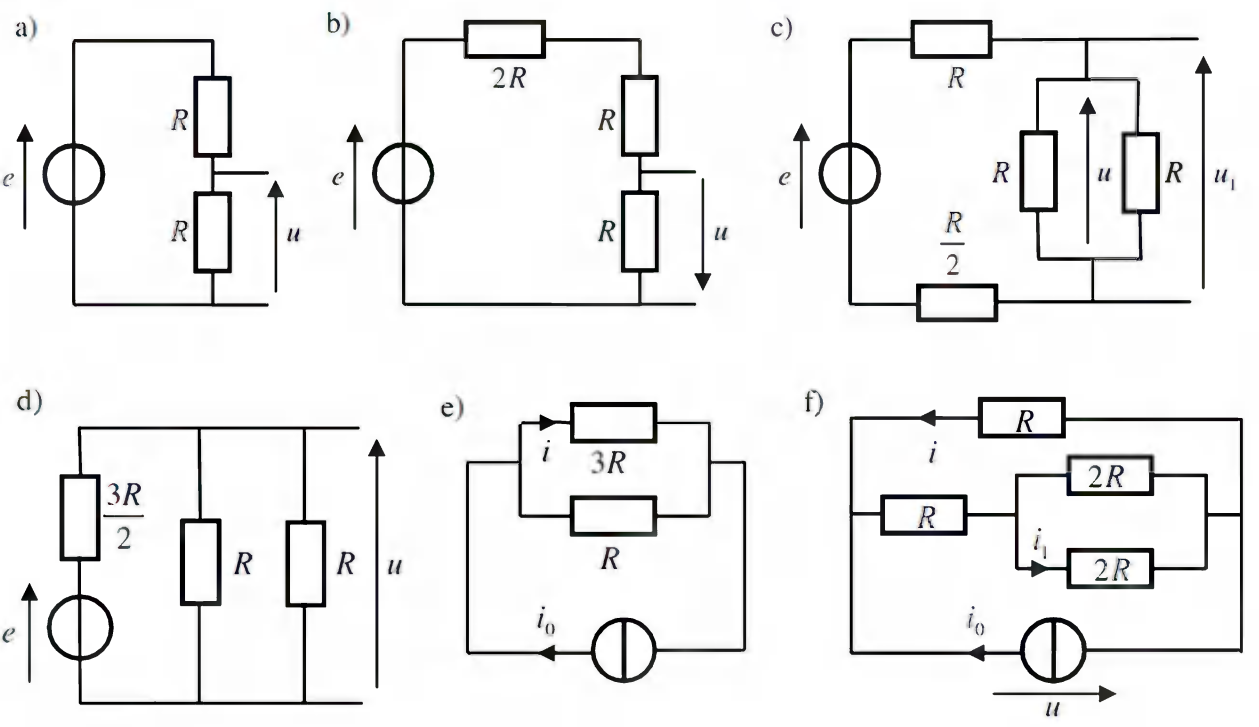
\includegraphics[width=\textwidth]{Images/exercicesKirchoff.png}

\subsection{Exercice 2}

\begin{minipage}[c]{\linewidth/2}
	\begin{circuitikz}
		%Circuit
		\draw (4, 0)
			to[short, i>=$I$] (2, 0)
			to[R, l=$R$] (0, 0)
			to[vsource, v_<=$e$] (0, -3)
			-- (4, -3);
		\draw (2, 0)
			to[R, l_=$R$, v^<=$U$] (2, -3);
	\end{circuitikz}
\end{minipage}%
\begin{minipage}[c]{\linewidth/2}
	On donne $R = \SI{10}{k\Omega}$.
	\begin{enumerate}
		\item Tracer la caractéristique du dipôle ci-contre.
		\item On ajoute une charge de résistance $R'=\SI{3}{k\Omega}$. Déterminer le point de fonctionnement de deux façons.
	\end{enumerate}
\end{minipage}

\subsection{Exercice 3 : Rendement d'un montage potentiométrique}

\begin{minipage}[c]{\linewidth/2}
	\begin{circuitikz}
		%Circuit
		\draw (0, 2)
		to[short, i>=$I$] (0, 3)
		--++(2, 0)
		to[R, l=$r_2$] ++(0, -2)
		to[R, l=$r_1$] ++(0, -2)
		--++(-2, 0)
		--++(0, 1)
		to[vsource, v=$E$] (0, 2);
		\draw (2, 1)
		to[short, i=$i_R$] ++(2, 0)
		to[R, l=$R$] ++(0, -2)
		--++(-2, 0);
	\end{circuitikz}
\end{minipage}%
\begin{minipage}[c]{\linewidth/2}
	Le rendement $\eta$ de ce diviseur de tension est le rapport $P_R$ de la puissance dissipée dans la résistance de charge $R$ à la puissance $P_E$ fournie par la source de tension $E$. Exprimer $\eta$ en fonction de $r_1$, $r_2$ et $R$.
	
	AN : $r_1 = \SI{750}{\Omega}$, $r_2=\SI{250}{\Omega}$, $R = \SI{80}{\Omega}$. Commentaire.
\end{minipage}

\subsection{Exercice 4 : Adaptation de puissance}

\begin{minipage}[c]{\linewidth/2}
	\begin{circuitikz}
		%Circuit
		\draw (0, 0)
		to[R, l=$R_0$] (3, 0)
		to[R, l=$R$] (3, -3)
		-- (0, -3)
		to[vsource, v=$E$] (0, 0);
	\end{circuitikz}
\end{minipage}%
\begin{minipage}[c]{\linewidth/2}
	Un générateur présente une tension à vide $E$ et une résistance interne $R_0$. On y branche une charge de résistance $R$. Pour quelle valeur de $R$ la puissance dissipée dans la résistance $R$ est elle maximale ? Que vaut alors cette puissance ?
\end{minipage}

\section{Semaine 02 (23/09-27/09) }


\e{Notions abordées :}
\begin{itemize}
	\item Circuits linéaires du premier ordre.
\end{itemize}

\subsection{Questions de cours}
\begin{enumerate}
	\item Relation entre la charge d'un condensateur et sa tension aux bornes.
	\item Relations entre intensité et tension pour un condensateur et une bobine.
	\item Continuité des grandeurs dans un circuit électrique.
	\item Établir l'expression de l'énergie stockée dans un condensateur/une bobine.
\end{enumerate}

\subsection{Exercice 1 : Résistance de fuite d'un condensateur}

Un condensateur réel présente des fuites de courants. Comment le modéliser ?

Il est inséré dans un circuit série comportant un générateur de f.é.m $E$, une résistance $r$ et un interrupteur $K$. On mesure la tension aux bornes du condensateur à l'aide d'un voltmètre idéal. On ferme $K$ et on attend que l'indication du voltmètre se stabilise. Puis on ouvre K en déclenchant au même instant un chronomètre. On constate que la tension indiquée par le voltmètre baisse de $10\%$ en un temps $T$.

On donne $E = \SI{1}{V}$, $r=\SI{10}{k\Omega}$, $T=\SI{1.0}{s}$ et $C=\SI{19}{\mu F}$.

\begin{enumerate}
	\item Exprimer la valeur $U$ vers laquelle la tension aux bornes du condensateur tend lorsque $K$ est fermé. En déduire une manière de déterminer $R_f$ (résistance de fuite).
	\item Montrer que la mesure du temps $T$ permet aussi de déterminer $R_f$. Commenter en relation avec l'une des hypothèses de l'énoncé.
\end{enumerate}

\subsection{Exercice 2 : Étude d'un circuit RL}

\begin{minipage}[c]{\linewidth/2}
	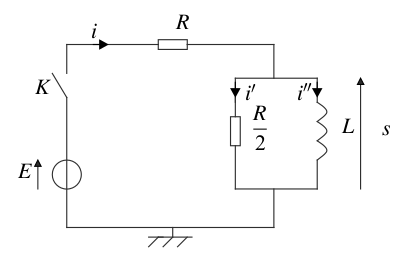
\includegraphics[width=\linewidth]{Images/mpsi_s02_ex02.png}
\end{minipage}%
\begin{minipage}[c]{\linewidth/2}
	À $t=0^-$, on ferme l'interrupteur $K$.
	\begin{enumerate}
		\item Donner $i$, $i'$, $i''$ et $s$ en $t=0^+$.
		\item Que vaut $s(t)$ lorsque $t$ tend vers l'infini.
		\item Établir l'équation différentielle vérifiée par $s(t)$.
		\item En déduire $s(t)$. En tracer l'allure.
		\item Exprimer le temps $t_0$ au bout duquel $s(t)$ a été divisé par $10$.
		\item On mesure $t_0=\SI{30}{\mu s}$ pour $R=\SI{1.0}{k\Omega}$. En déduire $L$.
	\end{enumerate}
\end{minipage}

\subsection{Exercice 3 : Rendement énergétique de la charge d'un condensateur}

On considère un circuit composé d'une résistance $R$ et d'un condensateur de capacité $C$ en série aux bornes duquel on place un générateur de tension idéal de f.é.m $E$ et un interrupteur $K$. À l'instant $t=0$, on ferme l'interrupteur $K$ et la tension $u_c$ aux bornes du condensateur est nulle.

\begin{enumerate}
	\item Établir l'équation différentielle vérifiée par $u_c$.
	\item Déterminer $u_c(t)$ et en tracer l'allure.
	\item Mêmes questions pour l'intensité du courant parcourant le circuit.
	\item Exprimer en fonction de $C$ et $E$ :
	\begin{itemize}
		\item L'énergie $\mathcal{E}_{elec}$ emmagasinée par le condensateur quand $t\rightarrow+\infty$.
		\item L'énergie $W_{Joule}$ dissipée par effet Joule dans la résistance entre $t=0$ et $t\rightarrow+\infty$.
		\item L'énergie $W_{gen}$ fournie par le générateur entre $t=0$ et $t\rightarrow+\infty$.
	\end{itemize}
	\item Donner une relation liant $\mathcal{E}_{elec}$, $W_{Joule}$ et $W_{gen}$ et proposer une interprétation physique de cette relation. Comment définir puis exprimer un rendement ?

\end{enumerate}
\section{Semaine 03 (30/09-04/10) }


\e{Notions abordées :}
\begin{itemize}
	\item Circuits linéaires du premier ordre (cf semaine précédente).
	\item Équilibre chimique.
\end{itemize}

\subsection{Questions de cours}
\begin{enumerate}
	\item Une mole de méthane réagit avec une mole de dioxygène selon une réaction de combustion. Déterminer la composition finale du système. (Équilibrer + Tableau d'avancement + Avancement final pour une réaction totale).
	\item Exprimer l'activité d'une espèce chimique dans un mélange. Préciser les hypothèses nécessaires.
	\item Exprimer le quotient réactionnel d'une réaction donnée et prévoir le sens d'évolution spontanée d'un système chimique.
\end{enumerate}

\subsection{Exercice 1 : Fluoration du dioxyde d'uranium}

Le dioxyde d'uranium solide réagit avec le fluorure d'hydrogène gazeux pour former du tétrafluorure d'uranium solide et de la vapeur d'eau. 

On maintient la température égale à $\SI{700}{K}$ et la pression totale à $\SI{1}{bar}$. La constante d'équilibre à $\SI{700}{K}$ est égale à $K^\circ = 6.8\times10^4$.

\begin{enumerate}
	\item Écrire la réaction.
	\item On part de $\SI{1.0}{mol}$ de dioxyde d'uranium et de $\SI{1.0}{mol}$ de fluorure d'hydrogène. Quelle sera la composition finale du système ?
	\item Même question en partant de $\SI{0.10}{mol}$ de dioxyde d'uranium et de $\SI{1.0}{mol}$ de fluorure d'hydrogène. Que remarque-t-on dans ce cas ?  
\end{enumerate}

\e{Réponses :}
\begin{enumerate}
	\item -
	\item $\xi = \SI{0.24}{mol}$.
	\item - 
\end{enumerate}

\subsection{Exercice 2 : Constante d'équilibre et quotient de réaction.}

Pour préparer industriellement du dihydrogène, on fait réagir en phase gazeuse du méthane avec de l'eau. La réaction produit également du monoxyde de carbone.

La réaction se déroule sous une pression totale constante $p_{tot} = \SI{10}{bar}$. La constante d'équilibre vaut $K^\circ = 15$. Initialement, le système contient $\SI{10}{mol}$ de méthane, $\SI{30}{mol}$ d'eau, $\SI{5}{mol}$ de monoxyde de carbone et $\SI{15}{mol}$ de dihydrogène. 

\begin{enumerate}
	\item Exprimer la constante d'équilibre en fonction des pressions partielles des constituants.
	\item Exprimer le quotient de réaction $Q$ en fonction de la quantité de matière de chacun des constituants et de la pression totale. Calculer $Q$ dans l'état initial.
	\item Le système est-il à l'équilibre thermodynamique ? Si non, dans quel sens se produira l'évolution ?
	\item Déterminer la composition du système à l'équilibre.
\end{enumerate}

\e{Réponses :}
\begin{enumerate}
	\item -
	\item $Q = 1.56$.
	\item -
	\item $\xi = \SI{3.6}{mol}$.
\end{enumerate}

\subsection{Exercice 3 : Utilisation du quotient de réaction.}

Un récipient de volume $V_0 = \SI{2.00}{L}$ contient initialement $\SI{0.500}{mol}$ de COBr$_2$ qui se décompose à une température de $\SI{346}{K}$ selon la réaction : $$\ce{COBr2_{(g)} = CO_{(g)} + Br2_{(g)}}$$.

\begin{enumerate}
	\item Déterminer la composition du système à l'équilibre sachant que la constante d'équilibre à $\SI{346}{K}$ vaut $K^\circ = 5.46$.
	\item Calculer le pourcentage de COBr$_2$ décomposé à cette température.
	\item L'équilibre précédent étant réalisé, on ajoute $\SI{2.00}{mol}$ de monoxyde de carbone. L'équilibre chimique est-il réalisé ? Si non, décrire l'évolution ultérieure du système.
\end{enumerate}

\e{Réponses :}
\begin{enumerate}
	\item $\xi = \SI{0.285}{mol}$.
	\item 57 \%.
	\item $Q = 43.2$, $\xi' = \SI{0.077}{mol}$.
\end{enumerate}
\section{Semaine 04 (07/10-11/10) }


\e{Notions abordées :}
\begin{itemize}
	\item Équilibre chimique (cf semaine précédente).
	\item Bases de l'optique géométrique.
\end{itemize}

\subsection{Questions de cours}
\begin{enumerate}
	\item Énoncer les lois de Snell-Descartes.
	\item Définir un rayon lumineux et un MTHI.
	\item Indice de réfraction ? Phénomène de réflexion totale ?
\end{enumerate}

\subsection{Exercice 1 : Réfractomètre de Pulrich}

\begin{minipage}[c]{\linewidth/2}
	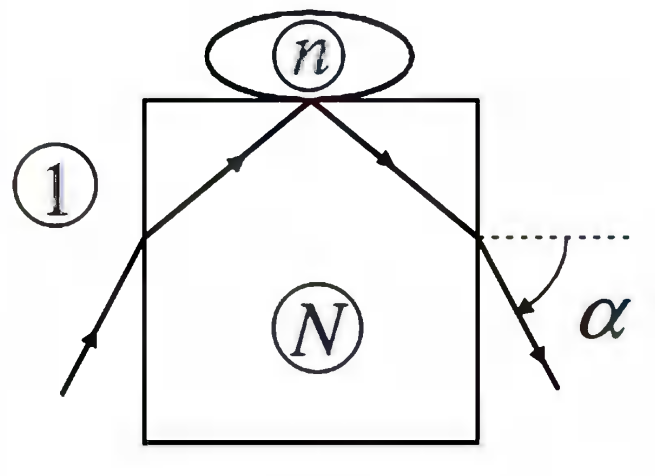
\includegraphics[width=\linewidth]{Images/mpsi_s04_ex01.png}
\end{minipage}%
\begin{minipage}[c]{\linewidth/2}
	Un réfractomètre de Pulrich est constitué d'un cube de verre d'indice $N$ connu sur lequel on a déposé une goutte d'un liquide d'indice $n$ inconnu. On observe un faisceau de rayons parallèles à la limite réfraction - réflexion totale et on mesure l'angle $\alpha$ correspondant. On donne $N=1.626$ et $\alpha=60$°.
\end{minipage} 

\begin{enumerate}
	\item Que vaut $n$ ?
	\item Quelles sont les valeurs mesurables de $n$ avec ce dispositif ?
\end{enumerate}

\e{Réponse} : $n = 1.376$

\subsection{Exercice 2}

\begin{minipage}[c]{\linewidth/2}
	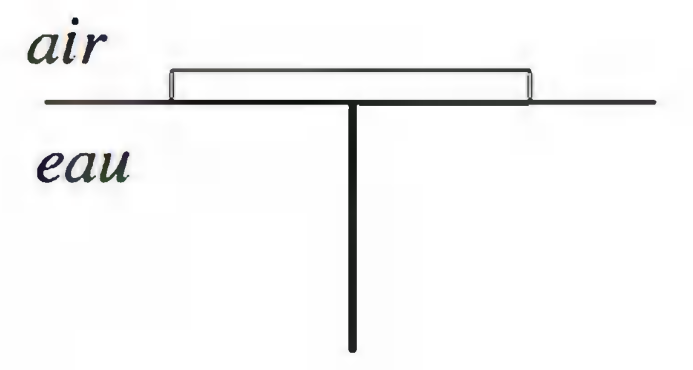
\includegraphics[width=\linewidth]{Images/mpsi_s04_ex02.png}
\end{minipage}%
\begin{minipage}[c]{\linewidth/2}
	Un disque en liège de diamètre $D = \SI{5}{cm}$ flotte sur l'eau. Il soutient une tige placée perpendiculairement en son centre. 
	
	Quelle est la longueur $h$ de la partie de la tige qu'un observateur dans l'air ne peut pas voir ?
\end{minipage}

\e{Réponse :} $h = \SI{2.1}{cm}$.

\subsection{Exercice 3 : Détection de pluie sur un pare-brise}

\begin{minipage}[c]{\linewidth/2}
	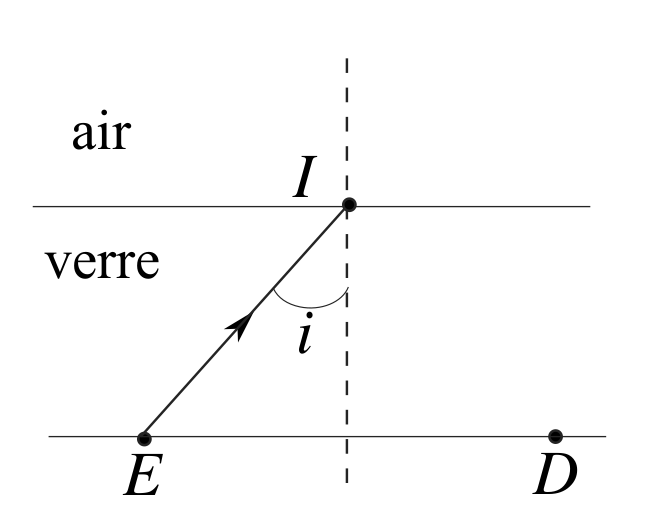
\includegraphics[width=\linewidth]{Images/mpsi_s04_ex03.png}
\end{minipage}%
\begin{minipage}[c]{\linewidth/2}
	On modélise un pare-brise par une lame de verre à faces parallèles, d'épaisseur $e = \SI{5}{mm}$, d'indice $n_v = 1.5$. Un fin pinceau lumineux issu d'un émetteur situé en $E$ arrive de l'intérieur du verre sur le dioptre verre/air en $I$ avec un angle d'incidence $i=60$°.
\end{minipage}

\begin{enumerate}
	\item Montrer que le flux lumineux revient intégralement sur le détecteur situé en $D$ et déterminer la distance $ED$.
	\item Comment ce dispositif permet-il de détecter un dépôt de pluie sur le pare-brise ? On supposera une épaisseur d'eau de $\SI{1}{mm}$.
\end{enumerate}

\e{Réponses :}
\begin{enumerate}
	\item $i_{lim} = 41.8$°.
	\item Distance au détecteur de $\SI{0.9}{cm}$.
\end{enumerate}



\chapter{MPI}

\section{Semaine 02 (23/09-27/09) }


\e{Notions abordées :}
\begin{itemize}
	\item Révisions de MPSI en électronique.
	\item Filtrage d'un signal périodique.
\end{itemize}

\subsection{Exercice 1}

\begin{minipage}[c]{\linewidth/3}
	\begin{circuitikz}
		%Circuit
		\draw (0, 0) 
		to[R, l=$R$] (3, 0)
		to [L, l=$L$, v<=$v_s$] ++ (0, -2)
		-- (0, -2)
		to [open, v=$v_e$] (0, 0);
	\end{circuitikz}
\end{minipage}%
\begin{minipage}[c]{\linewidth/2}
	On donne $R = \SI{1.0}{k\Omega}$ et $L = \SI{10}{mH}$.
	\begin{enumerate}
		\item Quel type de filtre ce circuit permet-il de réaliser ?
		\item Déterminer sa fonction de transfert.
		\item Déterminer les pentes des asymptotes en gain BF et HF.
		\item $v_e$ s'écrit comme somme de trois harmoniques de même amplitude, de même phase à l'origine et de fréquences respectives $f_1 = \SI{100}{Hz}$, $f_2 = \SI{1}{kHz}$ et $f_3 = \SI{100}{kHz}$. Écrire $v_e$ puis $v_s$.
		\item $v_e$ est maintenant un triangle de fréquence \SI{60}{Hz}. Quelle est la forme de $v_s$ ?
	\end{enumerate}
\end{minipage}

\subsection{Exercice 2}

\begin{minipage}[c]{\linewidth/2}
	\begin{circuitikz}
		%Circuit
		\draw (0, 0) 
		to[R, l=$R$] (3, 0)
		to[C, l=$C$] ++(2, 0)
		to [L, l=$L$, v<=$v_s$] ++ (0, -2)
		-- (0, -2)
		to [open, v=$v_e$] (0, 0);
	\end{circuitikz}
\end{minipage}%
\begin{minipage}[c]{\linewidth/2}
	\begin{enumerate}
		\item Quel type de filtre ce circuit permet-il de réaliser ?
		\item Déterminer sa fonction de transfert.
		\item Déterminer les pentes des asymptotes en gain BF et HF. Tracer le diagramme de Bode asymptotique.
		\item $v_e$ s'écrit comme somme de trois harmoniques de même amplitude, de même phase à l'origine et de fréquences respectives $f_1 = \SI{100}{Hz}$, $f_2 = \SI{1}{kHz}$ et $f_3 = \SI{100}{kHz}$. Écrire $v_e$ puis $v_s$.
		\item Ce filtre peut-il avoir un comportement dérivateur ? Intégrateur ?
	\end{enumerate}
\end{minipage}

\subsection{Exercice 3}

\begin{minipage}[c]{\linewidth/2}
	\begin{circuitikz}
		%Circuit
		\draw (0, 0) 
		to[R, l=$R$] (2, 0)
		to[C, l=$C$] ++(2, 0)
		to [R, l=$R$] ++ (0, -2)
		-- (0, -2)
		to [open, v=$v_e$] (0, 0);
		\draw (4, 0)
		-- (6, 0)
		to [C, l=$C$, v<=$v_s$] ++ (0, -2)
		-- (4, -2)
		;
	\end{circuitikz}
\end{minipage}%
\begin{minipage}[c]{\linewidth/2}
	On donne $R = \SI{1.0}{k\Omega}$ et $C = \SI{500}{nF}$.
	\begin{enumerate}
		\item Quel type de filtre ce circuit permet-il de réaliser ?
		\item Déterminer sa fonction de transfert.
		\item Déterminer la bande passante. Définir le facteur de qualité.
		\item $v_e$ s'écrit comme somme de trois harmoniques de même amplitude, de même phase à l'origine et de fréquences respectives $f_1 = \SI{100}{Hz}$, $f_2 = \SI{1}{kHz}$ et $f_3 = \SI{100}{kHz}$. Écrire $v_e$ puis $v_s$.
	\end{enumerate}
\end{minipage}


\section{Semaine 03 (30/09-04/10) }


\e{Notions abordées :}
\begin{itemize}
	\item Électronique de MPSI.
	\item Filtrage d'un signal périodique.
	\item Numérisation.
	\item Portes logiques.
\end{itemize}

\subsection{Exercice 1 : Intégration d'un créneau par un filtre passe bande}

Une tension créneau est injectée dans un filtre passe-bande non inverseur d'ordre 2, de pulsation de résonance $\omega_0$, de facteur de qualité $Q$ et de gain maximum $G_0$. La pulsation $\omega$ de la tension créneau est supposée grande devant $\omega_0$.

\begin{enumerate}
	\item Écrire la fonction de transfert du filtre.
	\item Montrer que ce filtre se comporte vis-à-vis du créneau d'entrée comme un intégrateur.
	\item Écrire l'équation différentielle reliant la tension d'entrée $v_e(t)$ et la tension de sortie $v_s(t)$ de l'intégrateur. Qu'obtient-on précisément en sortie du filtre ? Comment seraient modifiés les résultats si on ajoutait une tension continue au créneau à l'entrée ?
\end{enumerate}

\subsection{Exercice 2 : Shannon comme au cinéma}

Au cinéma, lorsqu'on regarde les roues d'une voiture qui démarre, on les voit d'abord tourner dans le sens réel puis elles semblent tourner à l'envers. Expliquer d'où provient cette illusion. Qu'observe-t-on en visionnant le film lorsque les roues de la voiture tournent à $f_1=\SI{1200}{tours/min}$ ? Et à $f_2 = \SI{1680}{tours/min}$.


\section{Semaine 04 (07/10-11/10) }


\e{Notions abordées :}
\begin{itemize}
	\item Électrocinétique.
	\item Mécanique de MPSI.
\end{itemize}

\subsection{Exercice 1 : Système à deux ressorts}

On considère une masse $m$ astreinte à se déplacer sur un axe horizontal $(Ox)$ et fixée à une paroi à gauche et une à droite par deux ressorts identiques $(k, l_0)$. Les parois sont distantes de $L$.

\begin{enumerate}
	\item Appliquer le principe fondamental de la dynamique à la masse $m$.
	\item En déduire la position d'équilibre $x_e$.
	\item Étudier les petites oscillations autour de la position d'équilibre.
	\item On envisage l'existence d'un frottement fluide d'intensité proportionnelle à la vitesse via une constante $\beta$. Établir l'équation différentielle du mouvement. Pour quelles valeurs de $\beta$ la masse $m$ oscille-t-elle ?
	\item Comment choisir $\beta$ pour un retour le plus rapide à la position d'équilibre. Quel est le temps caractéristique d'amortissement ?
\end{enumerate}

\subsection{Exercice 2 : Frottement et facteur de qualité}

On considère un ressort horizontal de constante de raideur $k$ et de longueur à vide $l_0$. Une extrémité du ressort est fixe et l'autre attachée à un mobile de masse $m$. Le mobile subit une force de frottement fluide proportionnelle à sa vitesse via une constante $\beta$.

\begin{enumerate}
	\item Déterminer l'équation différentielle du mouvement. Introduire une pulsation propre et un facteur de qualité.
	\item Résoudre l'équation différentielle. Simplifier l'expression dans le cas $Q \gg 1$.
	\item En déduire que $Q$ est une bonne approximation du nombre d'oscillations avant le retour à l'équilibre.
	\item On considère maintenant l'énergie mécanique relative perdue sur une pseudo-période. L'exprimer en fonction de $Q$. 
	\item On considère maintenant un opérateur qui impose une force $\vec{F(t)} = m A \cos{\omega t} \vec{e_x}$. Déterminer la fonction de transfert du système et interpréter $Q$ d'une nouvelle façon.
\end{enumerate}

\subsection{Exercice 3 : Mouvement autour d'une position d'équilibre}

Soit un point matériel de masse $m$ astreint à se déplacer selon un axe $(Ox)$ et d'énergie potentielle $E_p(x) = \frac{-a}{x^2} + \frac{b}{x^3}$ avec $a, b > 0$.

\begin{enumerate}
	\item Montrer en général qu'une position d'équilibre correspond à un extremum local d'énergie potentiel. À quelle condition une position d'équilibre est-elle stable ? instable ?
	\item Tracer le profil d'énergie potentiel.
	\item Déterminer la ou les position(s) d'équilibre ainsi que leur stabilité.
	\item Étudier les petites oscillations autour de la position d'équilibre stable.
	\item Déterminer, dans le cas d'une énergie potentielle générale, l'expression de la pulsation des petites oscillations.
\end{enumerate}


\chapter{MP}
\section{Semaine 01 (16/09-20/09) }


\e{Notions abordées :}
\begin{itemize}
	\item Révisions de MPSI en électronique.
	\item Filtrage d'un signal périodique.
	\item Traitement numérique du signal.
\end{itemize}

\subsection{Exercice 1}

\begin{minipage}[c]{\linewidth/3}
	\begin{circuitikz}
		%Circuit
		\draw (0, 0) 
			to[R, l=$R$] (3, 0)
			to [L, l=$L$, v<=$v_s$] ++ (0, -2)
			-- (0, -2)
			to [open, v=$v_e$] (0, 0);
	\end{circuitikz}
\end{minipage}%
\begin{minipage}[c]{\linewidth/2}
	On donne $R = \SI{1.0}{k\Omega}$ et $L = \SI{10}{mH}$.
	\begin{enumerate}
		\item Quel type de filtre ce circuit permet-il de réaliser ?
		\item Déterminer sa fonction de transfert.
		\item Déterminer les pentes des asymptotes en gain BF et HF.
		\item $v_e$ s'écrit comme somme de trois harmoniques de même amplitude, de même phase à l'origine et de fréquences respectives $f_1 = \SI{100}{Hz}$, $f_2 = \SI{1}{kHz}$ et $f_3 = \SI{100}{kHz}$. Écrire $v_e$ puis $v_s$.
		\item $v_e$ est maintenant un triangle de fréquence \SI{60}{Hz}. Quelle est la forme de $v_s$ ?
	\end{enumerate}
\end{minipage}

\subsection{Exercice 2}

\begin{minipage}[c]{\linewidth/2}
	\begin{circuitikz}
		%Circuit
		\draw (0, 0) 
		to[R, l=$R$] (3, 0)
		to[C, l=$C$] ++(2, 0)
		to [L, l=$L$, v<=$v_s$] ++ (0, -2)
		-- (0, -2)
		to [open, v=$v_e$] (0, 0);
	\end{circuitikz}
\end{minipage}%
\begin{minipage}[c]{\linewidth/2}
	\begin{enumerate}
		\item Quel type de filtre ce circuit permet-il de réaliser ?
		\item Déterminer sa fonction de transfert.
		\item Déterminer les pentes des asymptotes en gain BF et HF. Tracer le diagramme de Bode asymptotique.
		\item $v_e$ s'écrit comme somme de trois harmoniques de même amplitude, de même phase à l'origine et de fréquences respectives $f_1 = \SI{100}{Hz}$, $f_2 = \SI{1}{kHz}$ et $f_3 = \SI{100}{kHz}$. Écrire $v_e$ puis $v_s$.
		\item Ce filtre peut-il avoir un comportement dérivateur ? Intégrateur ?
	\end{enumerate}
\end{minipage}

\subsection{Exercice 3}

\begin{minipage}[c]{\linewidth/2}
	\begin{circuitikz}
		%Circuit
		\draw (0, 0) 
			to[R, l=$R$] (2, 0)
			to[C, l=$C$] ++(2, 0)
			to [R, l=$R$] ++ (0, -2)
			-- (0, -2)
			to [open, v=$v_e$] (0, 0);
		\draw (4, 0)
			-- (6, 0)
			to [C, l=$C$, v<=$v_s$] ++ (0, -2)
			-- (4, -2)
			;
	\end{circuitikz}
\end{minipage}%
\begin{minipage}[c]{\linewidth/2}
	On donne $R = \SI{1.0}{k\Omega}$ et $C = \SI{500}{nF}$.
	\begin{enumerate}
		\item Quel type de filtre ce circuit permet-il de réaliser ?
		\item Déterminer sa fonction de transfert.
		\item Déterminer la bande passante. Définir le facteur de qualité.
		\item $v_e$ s'écrit comme somme de trois harmoniques de même amplitude, de même phase à l'origine et de fréquences respectives $f_1 = \SI{100}{Hz}$, $f_2 = \SI{1}{kHz}$ et $f_3 = \SI{100}{kHz}$. Écrire $v_e$ puis $v_s$.
	\end{enumerate}
\end{minipage}
\section{Semaine 02 (23/09-27/09) }


\e{Notions abordées :}
\begin{itemize}
	\item Mécanique du point.
	\item Traitement numérique du signal.
\end{itemize}

\subsection{Exercice 1}

\begin{enumerate}
	\item Définir un satellite géostationnaire et calculer son altitude.
	\item Quel travail faut il fournir pour augmenter son altitude de $\SI{50}{km}$.
\end{enumerate}

\subsection{Exercice 2}

On considère un point matériel astreint à se déplacer autour d'un anneau en rotation autour d'un diamètre, à $\omega$ constante.

Positions d'équilibre ? Stabilité ?

\subsection{Exercice 3}

On cherche à graver sur un $CD$ une musique. Toutefois, il existe un signal parasite à $f_p = \SI{42.1}{kHz}$. 

\begin{enumerate}
	\item Échantillonnage sur 16 bits. Quelle est la taille du fichier si la durée vaut $74$ minutes.
	\item Le critère de Shannon est il vérifié ? Conséquence ?
	\item Comment résoudre ce problème ?
\end{enumerate}


\subsection{Exercice 4}

Décrire le mouvement d'une particule chargée dans un champ magnétique statique uniforme.

\section{Semaine 03 (30/09-04/10) }

\e{Notions abordées :}
\begin{itemize}
	\item Traitement numérique du signal.
	\item Mécanique de MPSI.
	\item Dynamique en référentiel non galiléen.
\end{itemize}

\subsection{Exercice 1}

Une tige rigide est en rotation uniforme autour de son axe à la pulsation $\omega$. Un mobile M est lié par un fil au point O situé sur l'axe à l'altitude $h$. 

\begin{enumerate}
	\item Démontrer la loi de composition des accélérations pour un référentiel en rotation uniforme.
	\item Déterminer l'angle $\alpha_0$ d'équilibre du mobile.
	\item Étudier la stabilité de la position d'équilibre.
\end{enumerate}

\subsection{Exercice 2}

Un électron et un proton de même énergie cinétique sont plongés dans un champ magnétique uniforme, orthogonal à leur vitesse initiale.

\begin{enumerate}
	\item Décrire qualitativement les trajectoires.
	\item Comparer :
	\begin{itemize}
		\item Leur vitesse.
		\item Le rayon de leur trajectoire.
		\item Leur période.
	\end{itemize}
	\item Calculer la force centrifuge subie par l'électron.
\end{enumerate}

\subsection{Exercice 3}

Un mobile $M$ coulisse sans frottement  sur un axe horizontal $(Ox)$ dans un train qui accélère avec une accélération $A\vec{u_x}$, le point $O$ étant fixé à l'arrière du wagon. Entre $O$ et $M$ on place un ressort $(k, l_0)$. À $t=0$, $x=l_0$ et la vitesse de $M$ dans le référentiel du train est nulle.

\begin{enumerate}
	\item Démontrer la loi de composition des accélérations dans un référentiel uniformément accéléré.
	\item Établir $x(t)$.
\end{enumerate}




\section{Semaine 04 (07/10-11/10) }

\e{Notions abordées :}
\begin{itemize}
	\item Mécanique de MPSI (forces centrales et dynamique du solide).
	\item Dynamique en référentiel non galiléen.
\end{itemize}

\subsection{Exercice 1 : Pendule pesant dans une voiture accélérée}

Une tige homogène de longueur $l$ et de masse totale $m$ est accrochée en un point $A$ du plafond d'une voiture. La voiture est en translation rectiligne d'accélération $a$ par rapport au référentiel terrestre supposé galiléen. 

Le moment d'inertie de la tige par rapport au point $A$ est $J = \frac{1}{3}m l ^2$. On admet que le point d'application de la force d'inertie d'entraînement est le centre d'inertie de la tige.

\begin{enumerate}
	\item Déterminer l'angle d'équilibre du pendule dans le référentiel de la voiture.
	\item Déterminer la période $T$ des petites oscillations du pendule autour de la position d'équilibre.
\end{enumerate}

\subsection{Exercice 2 : Limite de Roche}

\begin{minipage}[c]{\linewidth/2}
	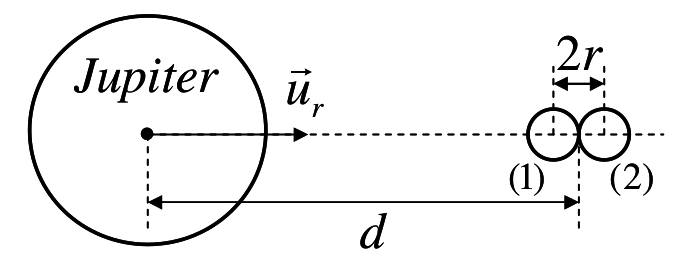
\includegraphics[width=\linewidth]{Images/mp_s04_ex02.png}
\end{minipage}%
\begin{minipage}[c]{\linewidth/2}
	On cherche à déterminer la distance en dessous de laquelle une comète s'approchant de Jupiter se sépare en plusieurs morceaux sous l'effet des forces de marée dues à Jupiter.
	
	On modélise la comète par deux sphères identiques de masses $m$ et de rayon $r$, alignées comme sur le dessin. On suppose que la comète est en orbite circulaire de rayon $d$ autour de Jupiter.
\end{minipage} 

\begin{enumerate}
	\item Montrer que le mouvement du centre d'inertie de la comète est uniforme. Quelle est la nature du mouvement du référentiel de la comète par rapport au référentiel de Jupiter ?
	\item Soit $\vec{R}$ la réaction de la sphère $(1)$ sur la sphère $(2)$. Dans le référentiel de la comète, appliquer le PFD à une des deux sphères.
	\item À quelle condition le contact entre les sphères est-il rompu ? Déterminer, sachant que $r \ll d$, la distance limite $d_{lim}$ en dessous de laquelle il ne peut exister de comètes.
\end{enumerate}

\e{Données :} $M_J = \SI{1.9e27}{kg}$, $R_J = \SI{7.1e4}{km}$ et masse volumique de la comète $\rho_c = \SI{1.0e3}{\kilogram\per\cubic\metre}$.

\e{Réponse :} $d_{lim} = \SI{1.8e5}{km}$.

\subsection{Exercice 3 : Usure d'une ligne de TGV}

Un train grande vitesse se dirige vers le sud, depuis Paris (latitude $48.8$°). On considère son mouvement dans le référentiel terrestre non galiléen. Montrer qu'apparaît une réaction horizontale de la voie sur le train. La comparer à la réaction verticale. 





\backmatter
% bibliography, glossary and index would go here.

\end{document}